\section{Results}

\begin{figure}[h]
    \centering
    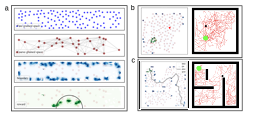
\includegraphics[width=0.9\textwidth]{figures/results_1.png}
    \caption{\textsc{Cognitive maps and agent behaviour} - \textbf{a}: \textit{place cells (PCs) over a rectangular environment, where the top plot report the node centers of the fine grained PCs, the top-center plot the node centers of coarse grained PCs together with their edges, the bottom-center instead
        shows the activity of the PCs tagged with the boundary neuromodulator over the coarse grained PCs, while the bottom plot shows the same but with the PCs tagged by the reward neuromodulator.} - 
    \textbf{b}: \textit{square environment, the right plot is the agent's trajectory (red) and reward area (green), the left plot si the \textit{cognitive map}, defined as overlay of the coarse-grain PCs, boundary and reward-sensitive PCs.} -
    \textbf{c}: \textit{square environment with internal walls, the right and left plot as before, but with the addition of the path planned by the agent to reach the target (grey)}}
    \label{fig:res1}
\end{figure}
